% ============================================================
% Sistema de Gestión de Inventario para Juguetería
% Documento en formato APA 7.ª edición
% Contexto: PHP + Laravel
% Motor: pdflatex (compilar 2 veces para el índice dinámico)
% ============================================================
\documentclass[12pt,letterpaper]{article}

\PassOptionsToPackage{quiet}{fontspec}

% ---------- Codificación y fuentes ----------
\usepackage[utf8]{inputenc}
\usepackage[T1]{fontenc}
\usepackage{lmodern}
\renewcommand{\familydefault}{\rmdefault}

% ---------- Idioma (español) ----------
\usepackage[spanish,es-tabla]{babel}
\usepackage[strict]{csquotes}

% ---------- Matemáticas ----------
\usepackage{amsmath,amssymb}

% ---------- Idiomas y enlaces ----------
\usepackage{xcolor}
\usepackage[hidelinks]{hyperref}
\usepackage{xurl}
\hypersetup{
  pdftitle={Sistema de Gestión de Inventario para Juguetería},
  pdfauthor={Simon Rodriguez Anculle, Gerar Rodrigo Camma Baldeon,
             Hugo Ernesto Florez Merma, Barry Valdivia Lovon,
             Samuel Llallacahi},
  colorlinks=true,
  linkcolor=blue,
  citecolor=blue,
  urlcolor=blue
}

% ---------- Geometría y espaciado (APA 7) ----------
\usepackage[margin=1in]{geometry}
\usepackage{setspace}
\doublespacing
\setlength{\parskip}{6pt}
\setlength{\parindent}{0pt}
\setlength{\emergencystretch}{3em}

% ---------- Encabezado con número de página (APA 7) ----------
\usepackage{fancyhdr}
\setlength{\headheight}{14.5pt}
\addtolength{\topmargin}{-2.5pt}
\pagestyle{fancy}
\fancyhf{}
\fancyhead[R]{\thepage}
\renewcommand{\headrulewidth}{0pt}

% ---------- Títulos de secciones estilo APA ----------
\usepackage{titlesec}
\titleformat{\section}
  {\normalfont\bfseries\centering}{}{0pt}{}
\titlespacing*{\section}{0pt}{12pt}{6pt}
\titleformat{\subsection}
  {\normalfont\bfseries}{}{0pt}{}
\titlespacing*{\subsection}{0pt}{12pt}{6pt}

% ---------- Gráficos e imágenes ----------
\usepackage{graphicx}
\graphicspath{{./media/}}
\usepackage{caption}
\captionsetup[figure]{labelsep=period, font=small, skip=6pt, justification=centering}
\usepackage{booktabs}
% \usepackage{array}

% ---------- Índice (TOC funcional) ----------
\setcounter{tocdepth}{2}

% ============================================================
\begin{document}

% ============================================================
% PORTADA
% ============================================================
\thispagestyle{empty}
\begin{center}
  \vspace*{1.2cm}
  
\includegraphics[width=4.5cm]{image1.png}

  \vspace{1.6cm}
  {\LARGE\bfseries Sistema de Gestión de Inventario\\[0.3em] para Juguetería}\\[2.0cm]

  {\large Simon Rodriguez Anculle\\
  Gerar Rodrigo Camma Baldeon\\
  Hugo Ernesto Florez Merma\\
  Barry Valdivia Lovon\\
  Samuel Llallacahi}\\[2.2cm]

  {\large Curso/Asignatura: Programación orientada a objetos\\[0.4cm]
  Docente: Luis Ignacio Diaz Bravo\\[0.4cm]
  Ciclo / Grado: 2do Ciclo - 2026}\\[1.8cm]

  {\large TECSUP}\\[0.3cm]
  {\large Arequipa, Perú}\\[0.3cm]
  {\large 2026}
\end{center}

\newpage

% ============================================================
% ÍNDICE FUNCIONAL
% ============================================================
\pagenumbering{arabic}
\tableofcontents
\newpage

% ============================================================
% RESUMEN
% ============================================================
\section*{Resumen}
\addcontentsline{toc}{section}{Resumen}

El presente proyecto de investigación expone el desarrollo de un Sistema de
Gestión de Inventario para una juguetería minorista, diseñado bajo el
paradigma de la Programación Orientada a Objetos (POO) empleando el lenguaje
PHP a través del framework \emph{Laravel}. La propuesta surge ante las
deficiencias identificadas en el control manual de existencias y la falta de
sincronización en tiempo real, lo cual impacta negativamente la rentabilidad
empresarial. A través de una arquitectura \emph{Modelo-Vista-Controlador}
(MVC) que implementa el mapeo objeto-relacional \emph{Eloquent ORM} y las
plantillas de vista \emph{Blade}, se ofrece una aplicación web modular,
escalable y altamente portable. La persistencia estructurada y el control
jerárquico por categorías y marcas aseguran la integridad de los datos,
optimizando las auditorías y permitiendo una toma de decisiones informada
basada en reportes automatizados.

\textbf{Palabras clave:} inventario, Programación Orientada a Objetos, PHP,
Laravel, Eloquent, juguetería.

\newpage

% ============================================================
% PROBLEMÁTICA
% ============================================================
\section{Problemática}

La gestión de inventarios en una juguetería minorista enfrenta desafíos
críticos debido a la alta rotación de productos y la diversidad de categorías
que deben administrarse. Actualmente, el uso de métodos manuales o registros en
hojas de cálculo aisladas ha evidenciado limitaciones estructurales en el
modelo operativo (Welling y Thompson, 2017). Esta práctica convencional genera
tres problemas operativos fundamentales que afectan la rentabilidad y la
eficiencia del negocio:

\begin{itemize}
  \item \textbf{Deficiencia en el control de stock por categorías y marcas:}
        la ausencia de una clasificación sistematizada impide una organización
        jerárquica eficiente, dificultando la localización y el seguimiento de
        juguetes según su fabricante o grupo de edad.
  \item \textbf{Invisibilidad de existencias en tiempo real:} la falta de
        sincronización entre las ventas realizadas y el registro de almacén
        imposibilita conocer la disponibilidad inmediata de los productos.
  \item \textbf{Ineficiencia en procesos manuales e inventarios físicos:}
        el procesamiento manual de ventas y la ejecución de auditorías físicas
        periódicas consumen recursos humanos de forma excesiva.
\end{itemize}

% ============================================================
\section{Importancia de la Solución}

El Sistema de Gestión de Inventario para juguetería resolverá la fragmentación
de datos mediante la centralización de operaciones en una aplicación web
nativa e independiente basada en el paradigma de la Programación Orientada a
Objetos (POO) mediante el framework Laravel (Stauffer, 2019). Al prescindir de
dependencias de escritorio pesadas, la solución garantiza agilidad, control
preciso de existencias y portabilidad, requiriendo únicamente un servidor web
con PHP y un gestor de base de datos MySQL.

% ============================================================
\section{Delimitación de Objetivos}

\subsection{Objetivo General}

Desarrollar una aplicación web utilizando PHP y Laravel que automatice la
gestión de inventario de una juguetería, optimizando el control de productos,
stock y categorías mediante una arquitectura modular orientada a objetos que
garantice la integridad y persistencia de la información.

\subsection{Objetivos Específicos}

\begin{itemize}
  \item Modelar el dominio del negocio de la juguetería mediante los pilares
        de la POO (Abstracción, Encapsulamiento, Herencia y Polimorfismo).
  \item Diseñar e implementar una capa de persistencia relacional robusta
        mediante \emph{Eloquent ORM} sobre un motor de base de datos MySQL.
  \item Construir una interfaz web moderna y modular con las plantillas
        \emph{Blade}, HTML5, CSS y JavaScript.
\end{itemize}

% ============================================================
\section{Marco Teórico}

Para fundamentar la construcción del software bajo estándares técnicos de la
industria, se describen las tecnologías y conceptos asociados a PHP y Laravel
que constituirán la estructura del sistema (PHP Documentation Group, 2024):

\begin{description}
  \item[PHP:] lenguaje de scripting del lado del servidor que provee un motor
        de ejecución síncrono, la gestión de memoria y las APIs estándares
        de control de datos sin requerir servidores externos.
  \item[Laravel:] framework MVC para PHP que facilita el desarrollo de
        aplicaciones web mediante \emph{rutas}, \emph{controladores} y
        \emph{migraciones} de base de datos (Stauffer, 2019).
  \item[Herencia y Polimorfismo:] mecanismos de POO que se emplearán para
        definir una clase base denominada ``Producto'' y especializar
        comportamientos mediante subclases (Welling y Thompson, 2017).
  \item[Eloquent ORM:] mapeo objeto-relacional de Laravel que actúa como
        puente de comunicación directo con el motor de base de datos
        relacional MySQL.
  \item[Blade \& Bootstrap:] motor de plantillas de Laravel combinado con el
        framework CSS Bootstrap para la maquetación de la interfaz web.
\end{description}

% ============================================================
\section{Ingeniería de Requerimientos}

Esta sección detalla los casos de uso, los trabajadores y las entidades clave del negocio para la juguetería.

\subsection{Casos de Uso del Negocio}

Las tablas a continuación resumen los cuatro casos de uso principales del sistema.

\begin{table}[htbp]
  \centering
  \caption{Caso de uso: Registrar venta}
  \begin{tabular}{p{4cm}p{11cm}}
    \toprule
    Caso & Registrar Venta \\
    \midrule
    Descripción & Permite al vendedor procesar la salida de productos solicitados por el cliente dentro del sistema de inventario. \\
    \midrule
    Precondición & El usuario (vendedor o cajero) debe haber iniciado sesión y el cliente debe haber seleccionado los juguetes a comprar con stock disponible. \\
    \midrule
    Secuencia & 
    1. El vendedor ingresa la opción de registrar venta en el sistema. \newline
    2. El vendedor selecciona o ingresa los productos solicitados por el cliente. \newline
    3. El sistema valida el stock disponible de los juguetes. \newline
    4. El vendedor confirma la transacción de venta. \newline
    5. El sistema procesa el registro de la venta y ejecuta de manera automática la actualización del inventario. \newline
    6. El sistema muestra un mensaje de confirmación de venta exitosa. \\
    \midrule
    Errores/Flujos alternativos & Stock insuficiente para la cantidad solicitada, error en la conexión o fallo al procesar el registro. \\
    \midrule
    Postcondición & La venta queda registrada en el sistema y el inventario de los juguetes vendidos se actualiza automáticamente. \\
    \midrule
    Objetivo & Agilizar el proceso de venta y mantener el nivel de stock actualizado en tiempo real en la tienda. \\
    \bottomrule
  \end{tabular}
  \par\vspace{1ex}
  \small Nota. Elaboración propia (2026).
\end{table}

\begin{table}[htbp]
  \centering
  \caption{Caso de uso: Gestionar abastecimiento}
  \begin{tabular}{p{4cm}p{11cm}}
    \toprule
    Caso & Gestionar abastecimiento \\
    \midrule
    Descripción & El proceso de cotizar, hacer el pedido al proveedor y recepcionar los nuevos juguetes. \\
    \midrule
    Precondición & El administrador identifica la necesidad de reponer stock en la tienda para evitar quiebres de inventario. \\
    \midrule
    Secuencia & 
    1. El administrador revisa el catálogo de productos y detecta baja disponibilidad o la necesidad de nuevos artículos. \newline
    2. El administrador cotiza los productos con el proveedor externo. \newline
    3. El administrador realiza y emite el pedido formal al proveedor. \newline
    4. El proveedor despacha y envía la nueva mercancía solicitada hacia la tienda. \newline
    5. El administrador o encargado de almacén recibe y recepciona los nuevos juguetes en el establecimiento. \newline
    6. El sistema o el administrador registra la entrada de la nueva mercancía para actualizar los niveles de stock. \\
    \midrule
    Errores/Flujos alternativos & Falta de stock en el proveedor, retraso en la entrega de la mercadería o discrepancias en la recepción de los juguetes. \\
    \midrule
    Postcondición & El inventario de la tienda es abastecido con los nuevos productos y los niveles de stock quedan actualizados. \\
    \midrule
    Objetivo & Mantener el stock de la tienda actualizado y evitar quiebres de inventario mediante una correcta provisión de mercancía. \\
    \bottomrule
  \end{tabular}
  \par\vspace{1ex}
  \small Nota. Elaboración propia (2026).
\end{table}

\begin{table}[htbp]
  \centering
  \caption{Caso de uso: Controlar inventario}
  \begin{tabular}{p{4cm}p{11cm}}
    \toprule
    Caso & Controlar inventario \\
    \midrule
    Descripción & El proceso interno de realizar auditorías, registrar mermas (juguetes rotos) y actualizar los niveles mínimos de stock. \\
    \midrule
    Precondición & El administrador o vendedor requiere verificar físicamente la mercancía y el estado del almacén de la tienda. \\
    \midrule
    Secuencia & 
    1. El administrador o vendedor accede al módulo de control de inventario. \newline
    2. Se realiza una auditoría física de los juguetes almacenados en la tienda. \newline
    3. Se identifican y registran las mermas o juguetes rotos encontrados durante la revisión. \newline
    4. Se actualizan los niveles mínimos de stock y los registros de existencias en el sistema. \newline
    5. El sistema guarda los cambios y emite un informe actualizado de inventario disponible. \\
    \midrule
    Errores/Flujos alternativos & Discrepancias entre el stock físico y el registrado en el sistema, o registro de mermas con datos erróneos. \\
    \midrule
    Postcondición & El inventario físico y del sistema coinciden, con las mermas registradas y los niveles de stock actualizados. \\
    \midrule
    Objetivo & Mantener la precisión de los registros de mercancía, prevenir pérdidas económicas y asegurar un control interno eficiente de la tienda. \\
    \bottomrule
  \end{tabular}
  \par\vspace{1ex}
  \small Nota. Elaboración propia (2026).
\end{table}

\begin{table}[htbp]
  \centering
  \caption{Caso de uso: Gestionar devoluciones y cambios}
  \begin{tabular}{p{4cm}p{11cm}}
    \toprule
    Caso & Gestionar devoluciones y cambios \\
    \midrule
    Descripción & El proceso desde que un cliente reporta un juguete defectuoso o desea cambiarlo, hasta que se resuelve con un cambio de producto o reembolso. \\
    \midrule
    Precondición & El cliente se presenta en el establecimiento con el juguete y el comprobante de pago correspondiente. \\
    \midrule
    Secuencia & 
    1. El cliente se acerca al vendedor para reportar un juguete defectuoso o solicitar un reembolso. \newline
    2. El vendedor recibe el producto y solicita el comprobante de la venta. \newline
    3. El vendedor verifica el estado del juguete y las condiciones de la devolución. \newline
    4. El vendedor procesa la solicitud seleccionando la opción de cambio de producto o reembolso. \newline
    5. El sistema actualiza el registro de inventario o genera la nota correspondiente según el caso. \newline
    6. Se entrega el nuevo producto o se efectúa el reembolso al cliente, concluyendo la atención. \\
    \midrule
    Errores/Flujos alternativos & Comprobante de pago inválido o inexistente, producto fuera del plazo permitido para devoluciones o juguete con daños ocasionados por el mal uso del cliente. \\
    \midrule
    Postcondición & La devolución o cambio queda registrado en el sistema y el inventario se ajusta de acuerdo con la solución aplicada. \\
    \midrule
    Objetivo & Atender de manera eficiente las incidencias de los clientes para garantizar satisfacción y mantener la correcta trazabilidad del inventario. \\
    \bottomrule
  \end{tabular}
  \par\vspace{1ex}
  \small Nota. Las tablas resumen los cuatro casos de uso del negocio incluyendo precondición, secuencia, etc.
\end{table}

\subsection{Trabajadores del Negocio}

\begin{table}[htbp]
  \centering
  \caption{Trabajadores del negocio}
  \begin{tabular}{p{4.5cm}p{10.5cm}}
    \toprule
    Trabajador & Descripción \\
    \midrule
    Vendedor & Atiende al cliente, realiza la venta y registra la salida del producto. \\
    \midrule
    Administrador/Dueño & Supervisa el negocio, gestiona el catálogo de productos, revisa reportes y realiza pedidos. \\
    \midrule
    Cajero & Recibe el pago del cliente, procesa la transacción y emite el comprobante de venta correspondiente. \\
    \midrule
    Encargado de almacén & Recibe y verifica la mercancía entregada por el proveedor, organiza físicamente el stock y actualiza los niveles de inventario en el sistema. \\
    \bottomrule
  \end{tabular}
  \par\vspace{1ex}
  \small Nota. Elaboración propia (2026).
\end{table}

\subsection{Entidades del Negocio}

\begin{table}[htbp]
  \centering
  \caption{Entidades del negocio}
  \begin{tabular}{p{4cm}p{11cm}}
    \toprule
    Entidades & Descripción \\
    \midrule
    Usuarios & Almacena la información de los usuarios internos del sistema que operan la tienda (Administrador y Vendedor), incluyendo sus credenciales de acceso y roles. \\
    \midrule
    Clientes & Contiene los datos de las personas que compran los juguetes (como su DNI, nombre completo, teléfono). \\
    \midrule
    Categorías & Clasifica los diferentes tipos de juguetes que ofrece el negocio. \\
    \midrule
    Inventario de Productos & Almacena la información detallada de los juguetes disponibles en la tienda (código, nombre, precio, stock, categoría a la que pertenece). \\
    \midrule
    Ventas & Registra las transacciones de venta realizadas, vinculando al cliente que realiza la compra y al usuario que la procesa, junto con la fecha y el monto total. \\
    \midrule
    Detalle\_ventas & Representa los ítems individuales incluidos en cada transacción de venta, especificando la cantidad de productos comprados, el precio unitario y el subtotal. \\
    \midrule
    Devoluciones & Registra las solicitudes de cambio o reembolso realizadas por los clientes, vinculando la venta original, el producto y la solución aplicada. \\
    \midrule
    Compras & Registra los pedidos realizados a un proveedor, vinculando al proveedor y al usuario que gestiona la compra, junto con la fecha y el monto total. \\
    \midrule
    Detalle\_compras & Representa los ítems individuales incluidos en cada compra, especificando el producto, la cantidad solicitada y el precio unitario. \\
    \bottomrule
  \end{tabular}
  \par\vspace{1ex}
  \small Nota. Un listado de entidad de negocio con campos de descripción para cada parte.
\end{table}

% ============================================================
\section{Diseño de la Solución}

\subsection{Diagrama de Clases UML (Estructura de Paquetes)}

Para asegurar la escalabilidad del sistema y cumplir con el Principio de
Responsabilidad Única (SRP), el código fuente se ha organizado estrictamente
separando las entidades de dominio frente a los componentes de infraestructura
técnica y la interfaz web (Larman, 2004). Como se observa en el diagrama de
clases, la arquitectura se divide en los siguientes paquetes principales:

\begin{itemize}
  \item \textbf{Models / Entidades:} representan las entidades del negocio
        (\emph{Cliente, Producto, Usuario, Venta} y \emph{DetalleVenta}),
        encapsulando sus atributos mediante los modelos de \emph{Eloquent}.
  \item \textbf{Controllers (MVC):} centralizan la lógica de negocio y las
        operaciones transaccionales hacia la base de datos (ej.
        \emph{ClienteController, ProductoController}), aislando las sentencias
        SQL del resto del sistema.
  \item \textbf{Views (Blade):} agrupan las plantillas web, donde la vista
        principal actúa como contenedor para enrutar hacia paneles como
        \emph{Ventas} o \emph{Productos}.
  \item \textbf{Database y Services:} proveen servicios transversales, como la
        conexión mediante \emph{Eloquent ORM}, el manejo de la sesión de
        usuario activo y herramientas como generación de tickets y utilidades
        de seguridad.
\end{itemize}

\begin{figure}[htbp]
  \centering
  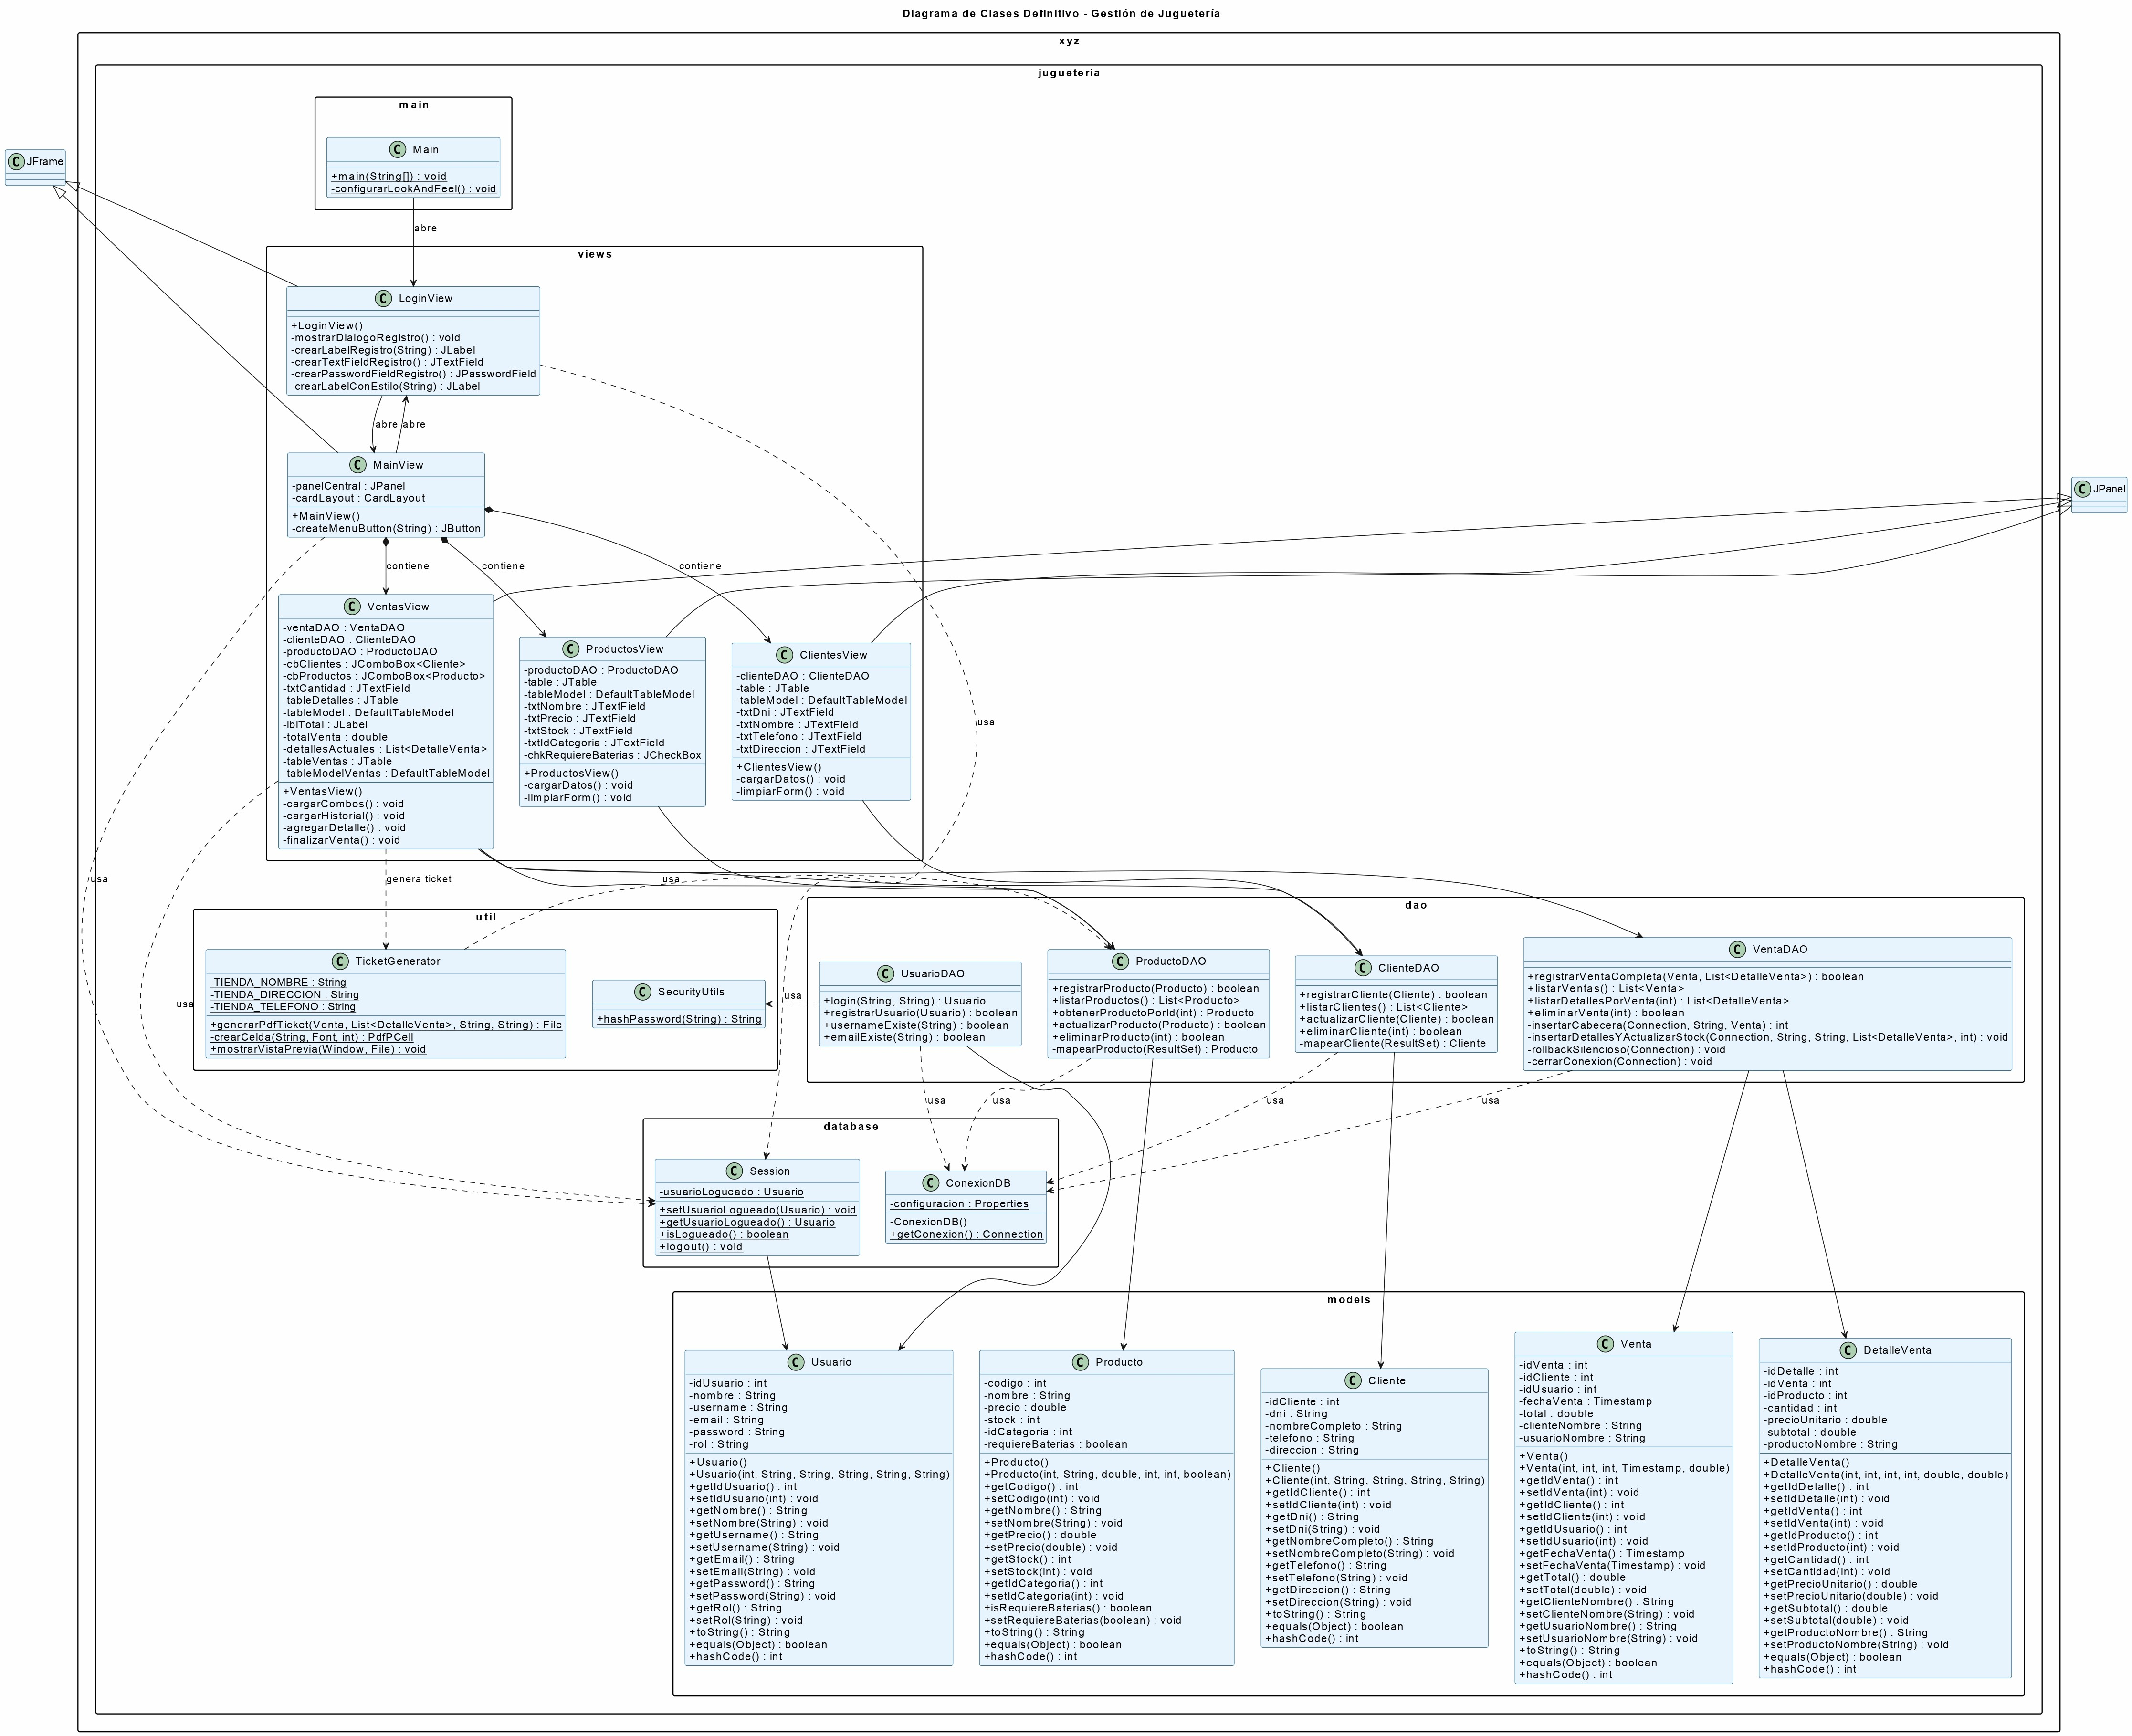
\includegraphics[width=0.9\textwidth]{image6.jpeg}
  \caption{Diagrama de clases UML: arquitectura y dependencias.}
\end{figure}

\subsection{Diagrama de Base de Datos (ERD Conceptual)}

El modelo entidad-relación (ERD) ha sido diseñado garantizando la integridad
referencial y la normalización de los datos. La arquitectura de la base de
datos se estructura en torno a las siguientes entidades clave y sus respectivos
tipos de datos:

\begin{itemize}
  \item \textbf{Tablas maestras:} entidades como \emph{usuarios},
        \emph{clientes} y \emph{categorias} que almacenan la información
        descriptiva y de acceso al sistema, utilizando llaves primarias
        auto-incrementables.
  \item \textbf{Gestión de inventario:} la tabla \emph{productos} centraliza el
        catálogo, stock (\emph{INT}) y precios (\emph{DECIMAL}), vinculándose
        directamente con su respectiva categoría mediante la llave foránea
        \emph{idCategoria}.
  \item \textbf{Núcleo transaccional:} compuesto por las tablas \emph{ventas}
        (cabecera) y \emph{detalle ventas} (cuerpo). La cabecera registra al
        responsable y al comprador mediante sus llaves foráneas, capturando la
        hora exacta (\emph{TIMESTAMP}). El detalle desglosa cada ítem vendido
        permitiendo calcular los subtotales con precisión monetaria
        (\emph{DECIMAL}) y mantener un historial de ventas exacto.
\end{itemize}

\begin{figure}[htbp]
  \centering
  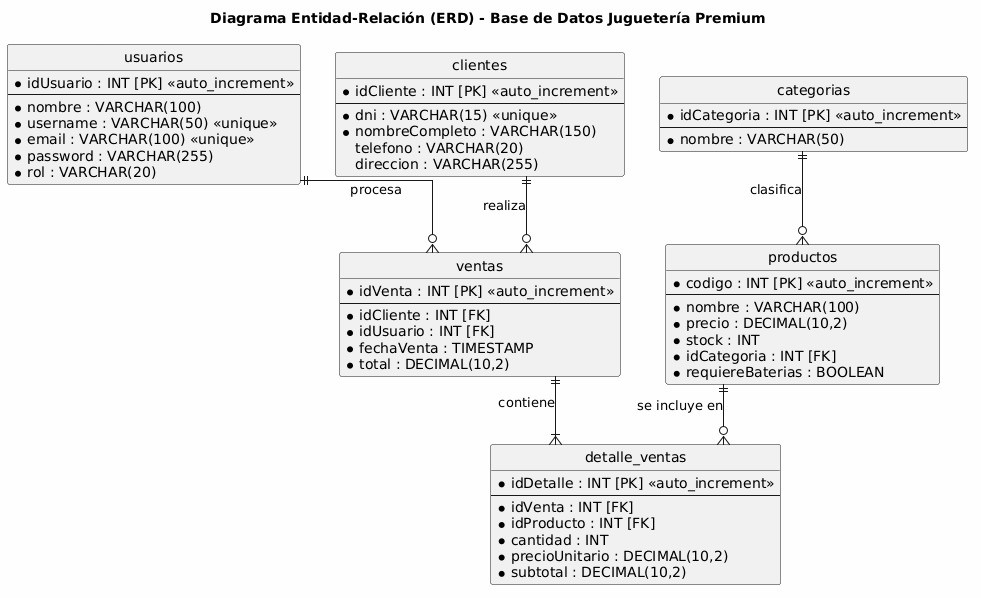
\includegraphics[width=0.85\textwidth]{image7.jpeg}
  \caption{Diagrama entidad-relación (ERD conceptual).}
\end{figure}


% ============================================================
\section{Estrategia de GIT y Repositorio}

El avance y control de versiones del proyecto se mantendrán de forma
transparente y colaborativa en la plataforma de alojamiento seleccionada. A la
fecha, el proyecto cuenta con un registro sólido de \textbf{commits} que
evidencian el trabajo constante y la integración de funcionalidades por parte
del equipo. Se configuró un archivo \emph{.gitignore} en la raíz del espacio de
trabajo para evitar la carga de metadatos locales de los entornos de desarrollo
(IDE), asegurando un repositorio limpio de código puro.

\begin{figure}[htbp]
  \centering
  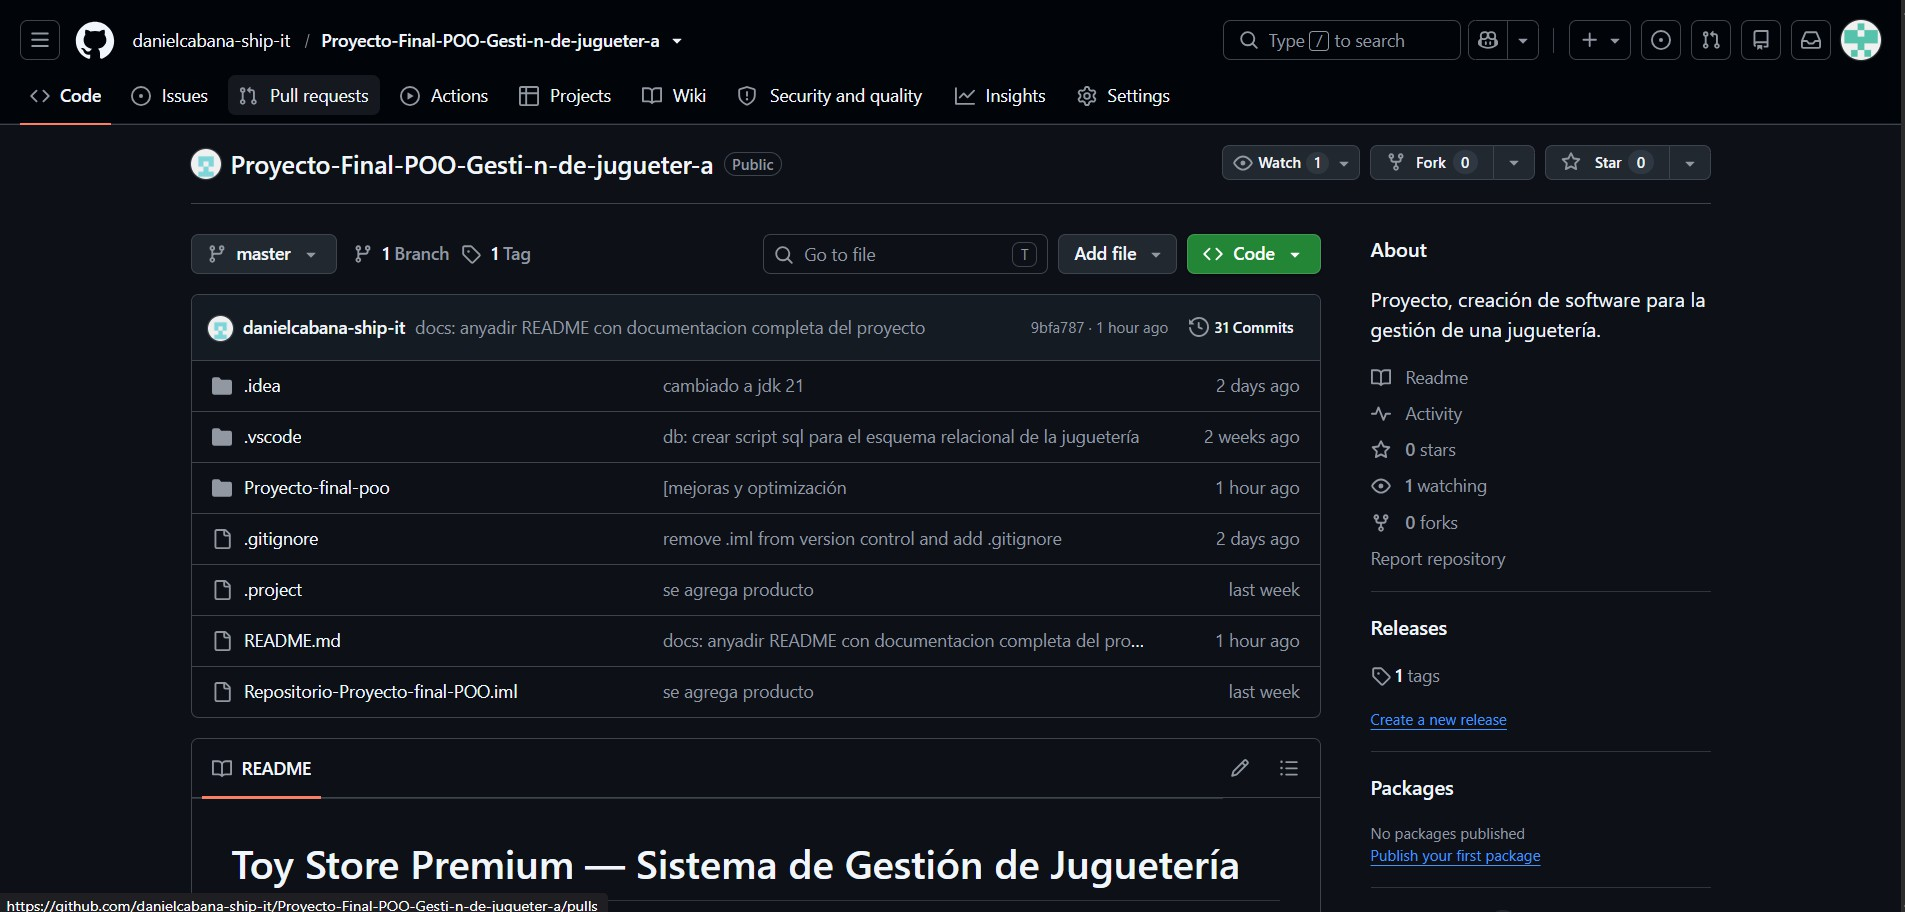
\includegraphics[width=0.85\textwidth]{image11.jpeg}
  \caption{Evidencia del repositorio en GitHub.}
\end{figure}

\subsection{Enlaces Importantes del Proyecto}

\begin{itemize}
  \item \textbf{Repositorio GitHub:}
        \href{https://github.com/danielcabana-ship-it/Proyecto-Final-POO-Gesti-n-de-jugueter-a}{Enlace
        al código fuente del proyecto}
\end{itemize}

% ============================================================
% REFERENCIAS (APA 7, con sangría francesa)
% ============================================================
\newpage
\section*{Referencias}
\addcontentsline{toc}{section}{Referencias}

\begin{thebibliography}{9}
  \setlength{\itemsep}{0pt}
  \setlength{\parskip}{0pt}

  \bibitem{welling2017}
  Welling, L., \& Thompson, L. (2017). \emph{PHP and MySQL web development}
  (5.\textsuperscript{a} ed.). Addison-Wesley Professional.

  \bibitem{stauffer2019}
  Stauffer, M. (2019). \emph{Laravel: Up and running} (2.\textsuperscript{a}
  ed.). O'Reilly Media.

  \bibitem{larman2004}
  Larman, C. (2004). \emph{Applying UML and patterns: An introduction to
  object-oriented analysis and design and iterative development}
  (3.\textsuperscript{a} ed.). Prentice Hall.

  \bibitem{php2024}
  PHP Documentation Group. (2024). \emph{Manual de PHP}.
  \url{https://www.php.net/manual/es/}

  \bibitem{bradshaw2019}
  S. Bradshaw, E. Brazil y C. Chodorow, \emph{MongoDB: The Definitive Guide: Powerful and Scalable Data Storage}, 3.ª ed., Sebastopol, CA, EE. UU.: O'Reilly Media, 2019.

  \bibitem{banker2016}
  K. Banker, P. Bakkum, S. Verch, D. Garrett y T. Hawkins, \emph{MongoDB in Action}, 2.ª ed., Shelter Island, NY, EE. UU.: Manning Publications, 2016.

  \bibitem{pressman2021}
  R. S. Pressman y B. R. Maxim, \emph{Ingeniería del software: Un enfoque práctico}, 9.ª ed., México: McGraw-Hill Education, 2021.

  \bibitem{wiegers2013}
  K. Wiegers y J. Beatty, \emph{Software Requirements}, 3.ª ed., Redmond, WA, EE. UU.: Microsoft Press, 2013.
\end{thebibliography}

\end{document}